
\documentclass[slidetop, 8pt, mathserif, unknownkeysallowed]{beamer}
\usepackage[frenchb]{babel}
\usepackage[T1]{fontenc}
\usepackage[utf8]{inputenc}
\usepackage{color, colortbl}
\usepackage{../res/tikz-uml}
%\usepackage[latin1]{inputenc}
\usetheme{Warsaw}        % Entre ces deux themes
%\usecolortheme{whale}   % mon coeur balance ...
\useoutertheme[width=50pt, height=30pt,left]{sidebar}
\usepackage{multimedia}
\useinnertheme[shadow=true]{rounded}
\usepackage{bookman}
\usepackage{multimedia}
\usepackage{../res/tikz-uml}
\usepackage{tikz}
\usepackage{calc}
\usepackage{xstring}
\usepackage{pgfopts}

%definecolor si 
 
\definecolor{white}{rgb}{1,1,1}
\definecolor{bleu}{RGB}{91,155,213}
\definecolor{orange}{RGB}{235,125,3}
\definecolor{vert}{RGB}{71,191,43}



\graphicspath{{../res/}}

\title{Présentation du projet PGP}
\author{O. Thibault, G. Leroy, M. Fin, P. Balmelle, \\B. Bouillie, I.Sory\,Barry, L.Barbay}
\institute{Université de Rouen}
\date{19 Janvier 2015}


\AtBeginSection[]
{
  \begin{frame}
  \frametitle{\color{white}Sommaire}
  \tableofcontents[currentsection,currentsubsubsection]
  \end{frame} 
}
\setbeamertemplate{footline}
{
  \leavevmode%
  \hbox{%
  \begin{beamercolorbox}[wd=.2\paperwidth,ht=2.25ex,dp=1ex,center]{institute in head/foot}%
    \usebeamerfont{institute in head/foot}\insertinstitute
  \end{beamercolorbox}%
  \begin{beamercolorbox}[wd=.6\paperwidth,ht=2.25ex,dp=1ex,center]{author in head/foot}%
    \usebeamerfont{author in head/foot}\insertauthor
  \end{beamercolorbox}%
  \begin{beamercolorbox}[wd=.2\paperwidth,ht=2.25ex,dp=1ex,right]{date in head/foot}%
    \usebeamerfont{date in head/foot}\insertshortdate{}\hspace*{2em}
    \insertframenumber{} / \inserttotalframenumber\hspace*{2ex} 
  \end{beamercolorbox}}%
  \vskip0pt%
}
\setbeamertemplate{background canvas}{
\includegraphics[width=\paperwidth,height=\paperheight]{fond.jpg}} % Width pour la largeur, height pour la hauteur de l'image
\setbeamertemplate{blocks}[rounded][shadow=true]

\begin{document}
 \begin{frame}
  \hfill
  
\includegraphics[scale=0.12]{logo_univ.png}
  \titlepage
\end{frame}

 \section{Intro}
\subsection{Contexte}
\subsection{L'équipe}

 \section{Le besoin}

\subsection{L'expression du besoin}

\begin{frame}
  \frametitle{\color{white} L'expression du besoin}
  une frame sur l'expression du besoin
\end{frame}

\begin{frame}
  \frametitle{\color{white} L'expression du besoin autre frame}
  une autre frame sur l'expression du besoin
\end{frame}


\subsection{Les exigences}

\begin{frame}
  \frametitle{\color{white} Les exigences}
  \begin{tikzpicture}

\umlactor[x=6]{Utilisateur}

\begin{umlsystem}[fill=red!10]{Interface graphique}
 \umlusecase[y=4, width=3cm]{Exécution d'actions GPG}
 \umlusecase[y=2, width=3cm]{Chiffrer/déchiffrer Signer/Vérifier}
 \umlusecase[y=0, width=3cm]{Affichage des commandes, des retours et des erreurs}
 \umlusecase[y=-2, width=3cm]{Choix du profil utilisateur}
 \umlusecase[y=-4, width=3cm]{Modification de la toile de confiance graphique}
\end{umlsystem}

\begin{umlsystem}[x=10, fill=red!10]{Attaque sur les KeyId}
 \umlusecase[width=3cm]{Calcul d'une seconde pré-image pour une clé donnée}
\end{umlsystem}

\umlassoc{Utilisateur}{usecase-1}
\umlassoc{Utilisateur}{usecase-2}
\umlassoc{Utilisateur}{usecase-3}
\umlassoc{Utilisateur}{usecase-4}
\umlassoc{Utilisateur}{usecase-5}
\umlassoc{Utilisateur}{usecase-6}

\end{tikzpicture}
\end{frame}

\begin{frame}
  \frametitle{\color{white} Les livrables}
  \begin{itemize}
   \item Rapport complet sur GnuPG et OpenPGP
   \item Interface graphique pour GnuPG
   \item Document d'utilisation de l'interface
   \item Rapport d'étude des limites cryptographiques de PGP
   \item Implémentation de l'attaque sur les KeyId
  \end{itemize}

\end{frame}

 \section{La Qualité}

	%						%
	%  PREMIERE PARTIE		%
	%						%

\subsection{Développement et tests}

% Première slide %
\begin{frame}
  \frametitle{\color{white} Déroulement du développement et des tests}
  Schéma de Matthieu ici

\end{frame}

% Deuxième slide %
\begin{frame}
  \frametitle{\color{white} Types de tests}
  \begin{itemize}
  \item Tests unitaires
  \item Tests d'intégration
  \item Tests de non-régression
  \item Tests d'acceptation
  \end{itemize}
  
  
\end{frame}


	%						%
	%  SECONDE PARTIE		%
	%						%

\subsection{Stratégie de test}
% Troisième slide %
\begin{frame}
  \frametitle{\color{white} Stratégies des tests}
  \begin{block}{Approche choisie pour les tests}
   Ecriture des tests automatisés puis écriture du code pour faire passer le test
  \end{block}
  \begin{figure}[p]
    \centering
    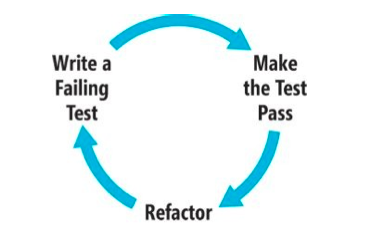
\includegraphics[scale=.25]{tests.png}
    \caption{Développement dirigé par les tests}
  \end{figure}
\end{frame}

% Quatrième slide %
\begin{frame}
  \frametitle{\color{white} Que mettre ici ?}
  

\end{frame}



 \section{La technique}

\subsection{Outils}
\begin{frame}
  \frametitle{\color{white} Outils de développement}
  \begin{block}{Langage}
    \begin{itemize}
      \item C++ 11.
      \item Qt 5.
      \hfill
      
\includegraphics[scale=.015]{Qt-logo.png}
    \end{itemize}
  \end{block}
  \begin{block}{Pourquoi le C++ 11 ?}
    \begin{itemize}
      \item Rapidité d'exécution.
      \item Communication simplifiée avec GPG.
      \item Langage natif de Qt.
    \end{itemize}
  \end{block}
  \begin{block}{Pourquoi Qt 5 ?}
    \begin{itemize}
      \item Cadriciel multiplate-forme.
      \item KDE est basé sur ce cadriciel.
    \end{itemize}
  \end{block}
\end{frame}

\subsection{Maquette}
\begin{frame}
  \frametitle{\color{white} Maquette}
  \begin{block}{Livrables}
    \begin{itemize}
      \item Livrable 1 : Gestion des clefs, vue des commandes.
      \item Livrable 2 : Éditeur/opérations cryptographiques.
      \item Livrable 3 : Toile de confiance.
    \end{itemize}
  \end{block}
  \begin{center}
    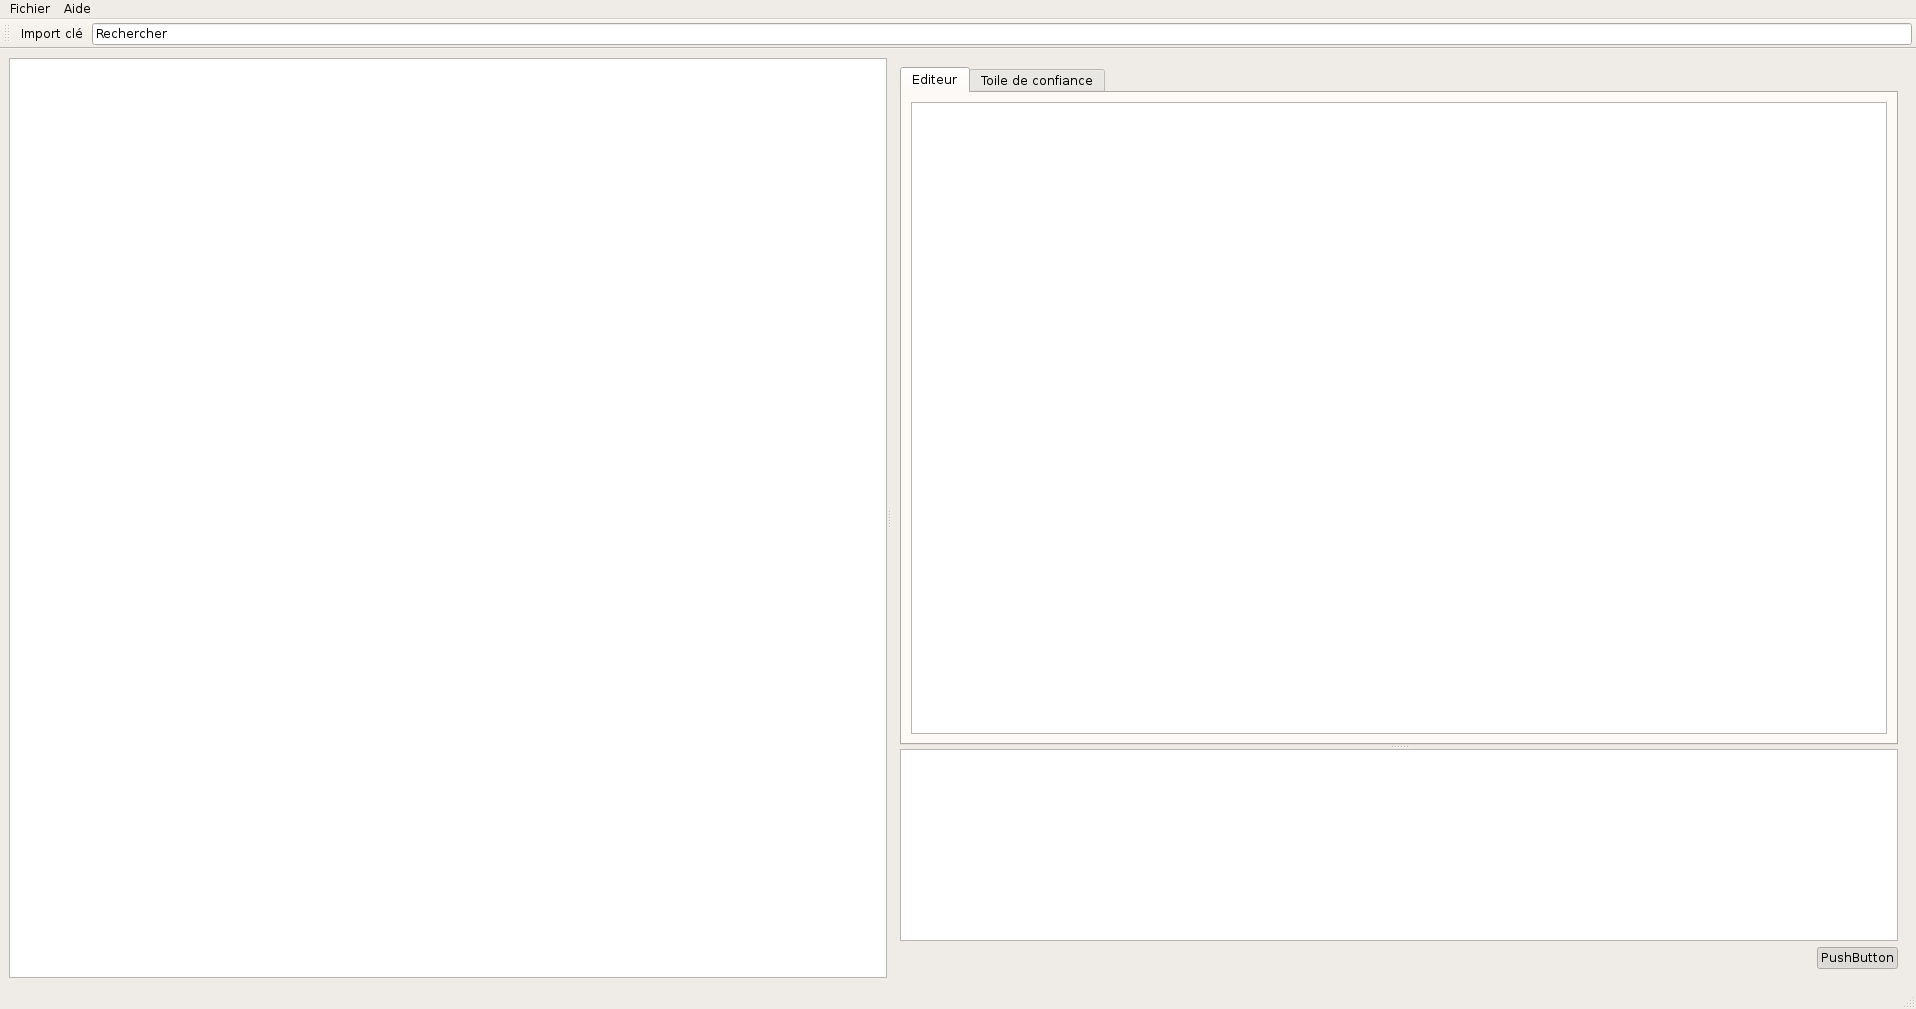
\includegraphics[scale=.14]{maquette.png}
  \end{center}
\end{frame}

\subsection{Procédés de gestion}
\begin{frame}
  \frametitle{\color{white} Procédés de gestion}
  \hfill
  
\includegraphics[scale=.05]{git-logo.png}
  \begin{center}
    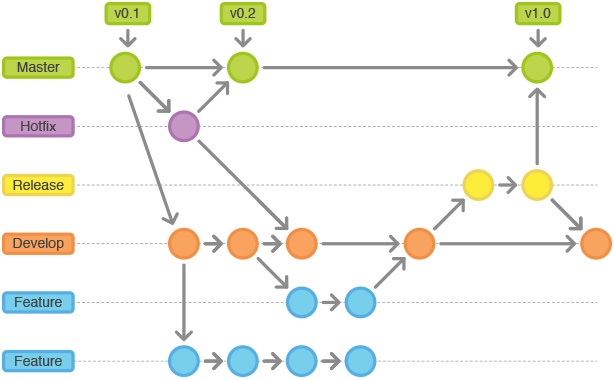
\includegraphics[scale=.45]{git_workflow}
  \end{center}
\end{frame}

\subsection{Risque}
\begin{frame}
  \frametitle{\color{white} Maîtrise des outils}
  \begin{block}{Prévention}
    \begin{itemize}
      \item Réalisation de séances de programmation C++/Qt.
      \item Réalisation de séances de découverte d'OpenPGP avec GnuPG.
    \end{itemize}
  \end{block}
  \begin{block}{Actions}
    \begin{itemize}
      \item Séances d'approfondissement des outils en continu.
      \item Ré-attribution des rôles en fonction des difficultés rencontrées.
    \end{itemize}
  \end{block}
\end{frame}


 \section{La gestion}
\subsection{La gestion...}
\begin{frame}
  \frametitle{\color{white} La quatilté 1ere frame}
  une frame sur l'expression du besoin
\end{frame}
\begin{frame}
  \frametitle{\color{white} La gestion autre frame}
  une autre frame sur la gestion
\end{frame}
\subsection{Une autre partie ...}
\begin{frame}
  \frametitle{\color{white} une frame sur l'autre partie.}
  frame
\end{frame}

 \section{Conclusion}
\begin{frame}
  \frametitle{\color{white}Conclusion}
  \begin{block}{Compétences acquises}
      \begin{itemize}
        \item Connaissance approfondie de GnuPG.
        \item Le langage C++ et Qt.
        \item Outils collaboratifs.
        \item Une première expérience de gestion de projet enrichissante.
      \end{itemize}
    \end{block}
\end{frame}
        

\end{document}

